\documentclass{beamer}
\usepackage[british]{babel}
\usepackage[utf8]{inputenc}
\usepackage{styles/jyumacros}
\usepackage[version=4]{mhchem}
\usepackage{textgreek}
\usepackage[texcoord]{eso-pic}
\usepackage[absolute,overlay]{textpos}
\usefolder{styles}
\usetheme{jyu}

%change these to your own logos if needed (try and match sizes, otherwise, change sizes in Outer Theme file).
\titlegraphic{assets/coverlogo.pdf} %logo on the cover page
\newcommand{\smalllogo}{assets/small_white.pdf} %small logo on frames

%Personal info---------------------------------------------
\title{The MARA-LEB RFQ Guide System}
\date{2021 Euroschool on Exotic Beams}
\author[auth]{Jorge Romero}
\institute[inst]{\vspace*{-1em}}
%----------------------------------------------------------

\begin{document}
\begin{frame}
\titlepage
\end{frame}

\begin{frame}{Motivation}
    \vspace*{4em}
    \begin{itemize}
        \item Studying the N=Z region of the nuclear chart 
        \begin{itemize}
            \item<2-> Test predictions of the nuclear shell model
            \item<3-> Increase understanding in the astrophysical rp process
        \end{itemize}
    \end{itemize}
    \vspace*{1em}
   
   \onslide<4->{ MARA-LEB will provide the required efficiency and
    
    selectivity to MARA, a high mass-resolving power
    
    separator in Jyväskylä's Accelerator Lab.}
    \flushright
    \vspace*{-5em}
    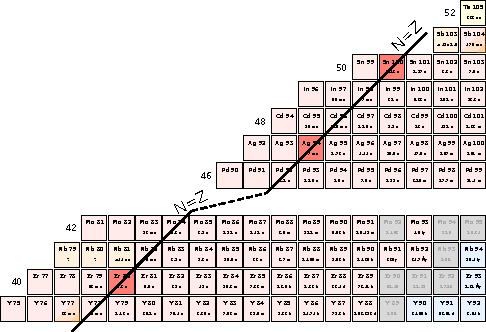
\includegraphics[scale=0.9]{assets/chart.pdf}
\end{frame}

\begin{frame}{Setup}
    \begin{textblock*}{0.8\paperwidth}(0.1\paperwidth,0.25\paperheight)
        \onslide<1>{The MARA-LEB Gas Cell is placed at MARA's focal plane.}
        
        \vspace*{2em}
        \centering
        \includegraphics<1>[scale=0.36]{assets/LEB_diagram1.pdf}
    \end{textblock*}
    
    \begin{textblock*}{0.8\paperwidth}(0.1\paperwidth,0.25\paperheight)
        \onslide<2>{Recoils from MARA are thermalised and neutralised by a buffer gas.}
        
        \vspace*{2em}
        \centering
        \includegraphics<2>[scale=0.36]{assets/LEB_diagram2.pdf}
    \end{textblock*}

    \begin{textblock*}{0.8\paperwidth}(0.1\paperwidth,0.25\paperheight)
        \onslide<3>{Recoils can be re-ionised using laser ionisation in the gas cell.}
        
        \vspace*{2em}
        \centering
        \includegraphics<3>[scale=0.36]{assets/LEB_diagram3.pdf}
    \end{textblock*}

    \begin{textblock*}{0.8\paperwidth}(0.1\paperwidth,0.25\paperheight)
        \onslide<4>{In-gas-jet laser ionisation can also be performed for better resolution.}
        
        \vspace*{2em}
        \centering
        \includegraphics<4>[scale=0.36]{assets/LEB_diagram4.pdf}
    \end{textblock*}

    \begin{textblock*}{0.8\paperwidth}(0.1\paperwidth,0.25\paperheight)
        \onslide<5>{Ions are confined and transported using radio-frequency quadrupole ion guides.}
        
        \vspace*{2em}
        \centering
        \includegraphics<5>[scale=0.36]{assets/LEB_diagram5.pdf}
    \end{textblock*}

    \begin{textblock*}{0.8\paperwidth}(0.1\paperwidth,0.25\paperheight)
        \onslide<6>{Ions are focused and accelerated to 30\,keV by extraction electrodes.}
        
        \vspace*{2em}
        \centering
        \includegraphics<6>[scale=0.36]{assets/LEB_diagram6.pdf}
    \end{textblock*}

    \begin{textblock*}{0.8\paperwidth}(0.1\paperwidth,0.25\paperheight)
        \onslide<7>{A magnetic dipole and an electrostatic deflector transport the ions vertically and provide further mass selection.}
        
        \vspace*{2em}
        \centering
        \includegraphics<7>[scale=0.36]{assets/LEB_diagram7.pdf}
    \end{textblock*}

    \begin{textblock*}{0.8\paperwidth}(0.1\paperwidth,0.25\paperheight)
        \onslide<8>{The ions are finally transported to detectors.}
        
        \vspace*{2em}
        \centering
        \includegraphics<8>[scale=0.36]{assets/LEB_diagram8.pdf}
    \end{textblock*}
\end{frame}

\begin{frame}{Simulations}
    \vspace*{2em}
    \centering
    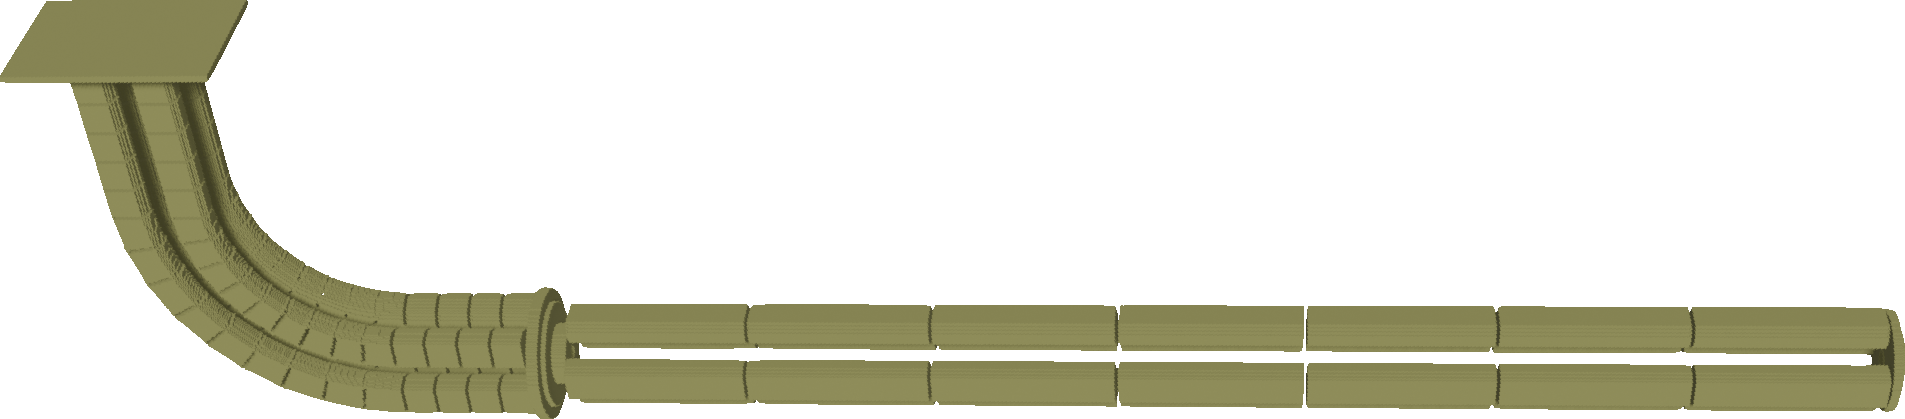
\includegraphics[scale=0.3]{assets/RFQguides.pdf}

    \vfill
    \begin{flushleft}
        Simulations of transmission efficiency through the RF guides in terms of applied voltages was performed in Simion.
    \end{flushleft}
\end{frame}

\begin{frame}{Simulations}
    \vspace*{2em}
    \flushright
    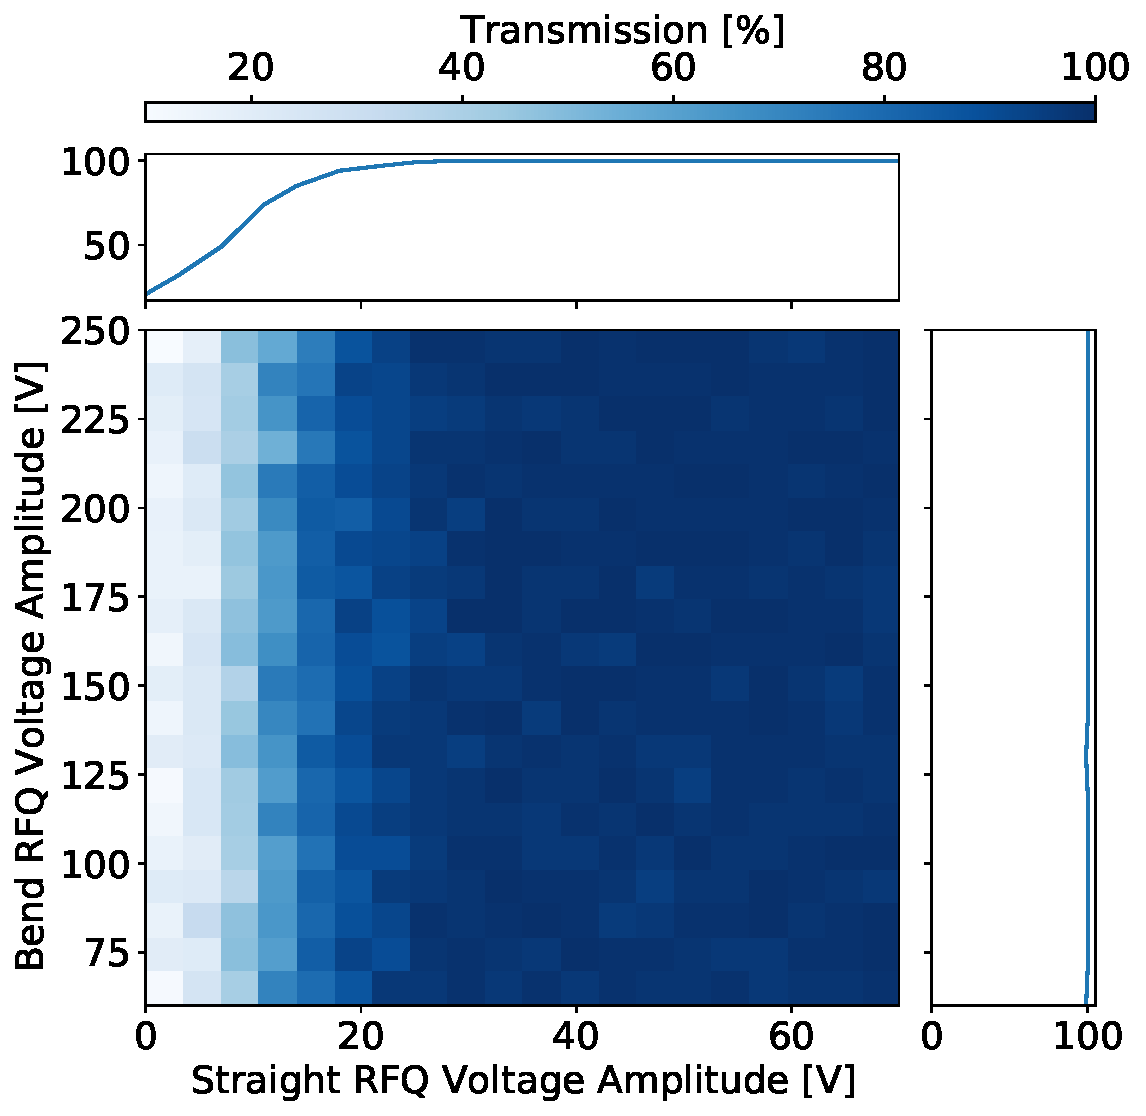
\includegraphics[scale=0.4]{assets/newgeo.pdf}

    \begin{textblock*}{0.2\paperwidth}(0.1\paperwidth,0.4\paperheight)
        \flushleft
        Optimal working voltages were determined. 
    \end{textblock*}
\end{frame}

\begin{frame}{Simulations}
    \vspace*{3em}

    \begin{center}  
        A new geometry for a differential pumping section aperture was tested.
    \end{center}

    \begin{center}  
        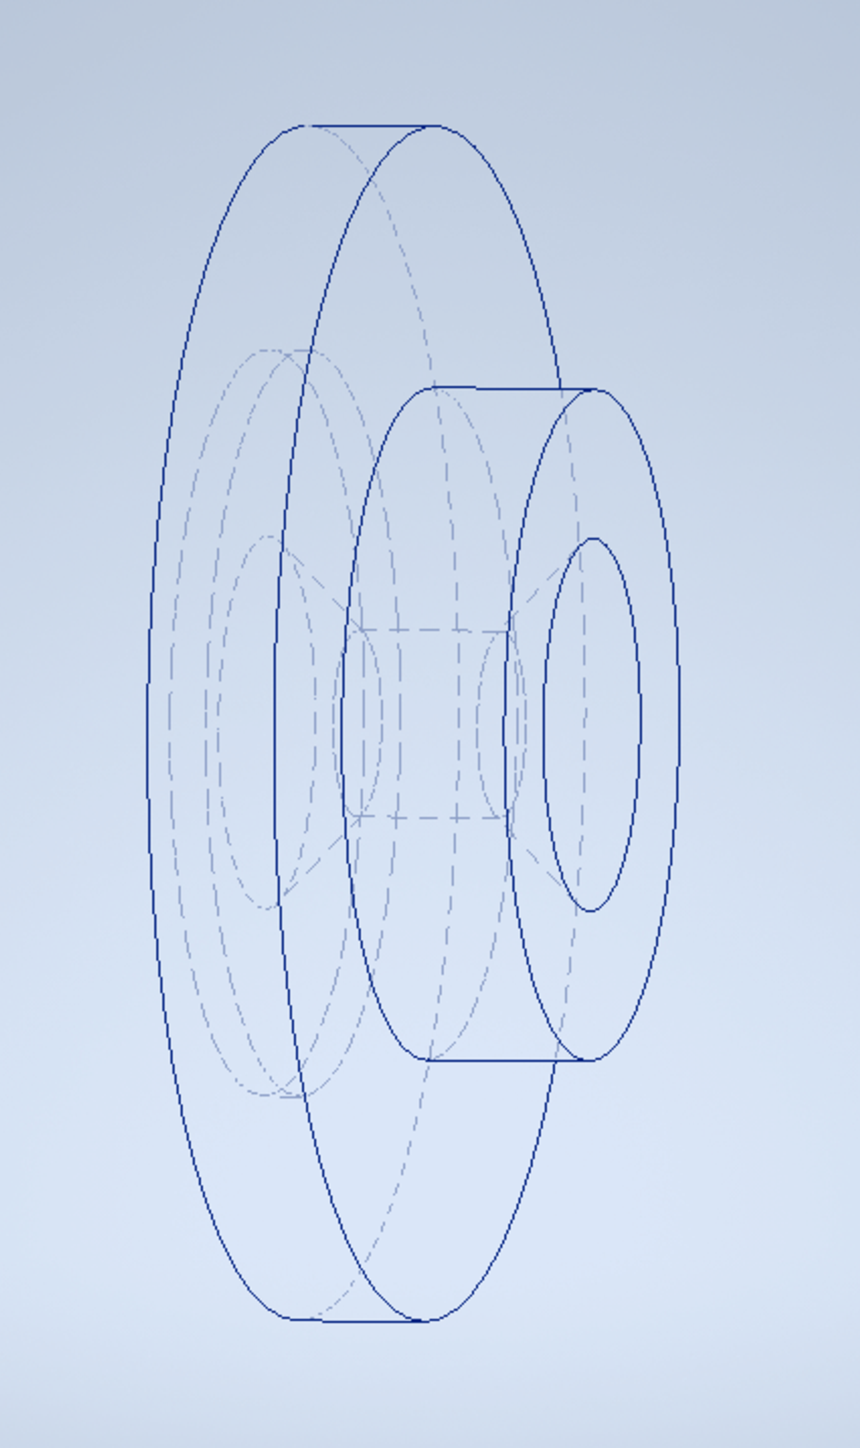
\includegraphics[scale=0.2]{assets/oldchamfer.pdf}
        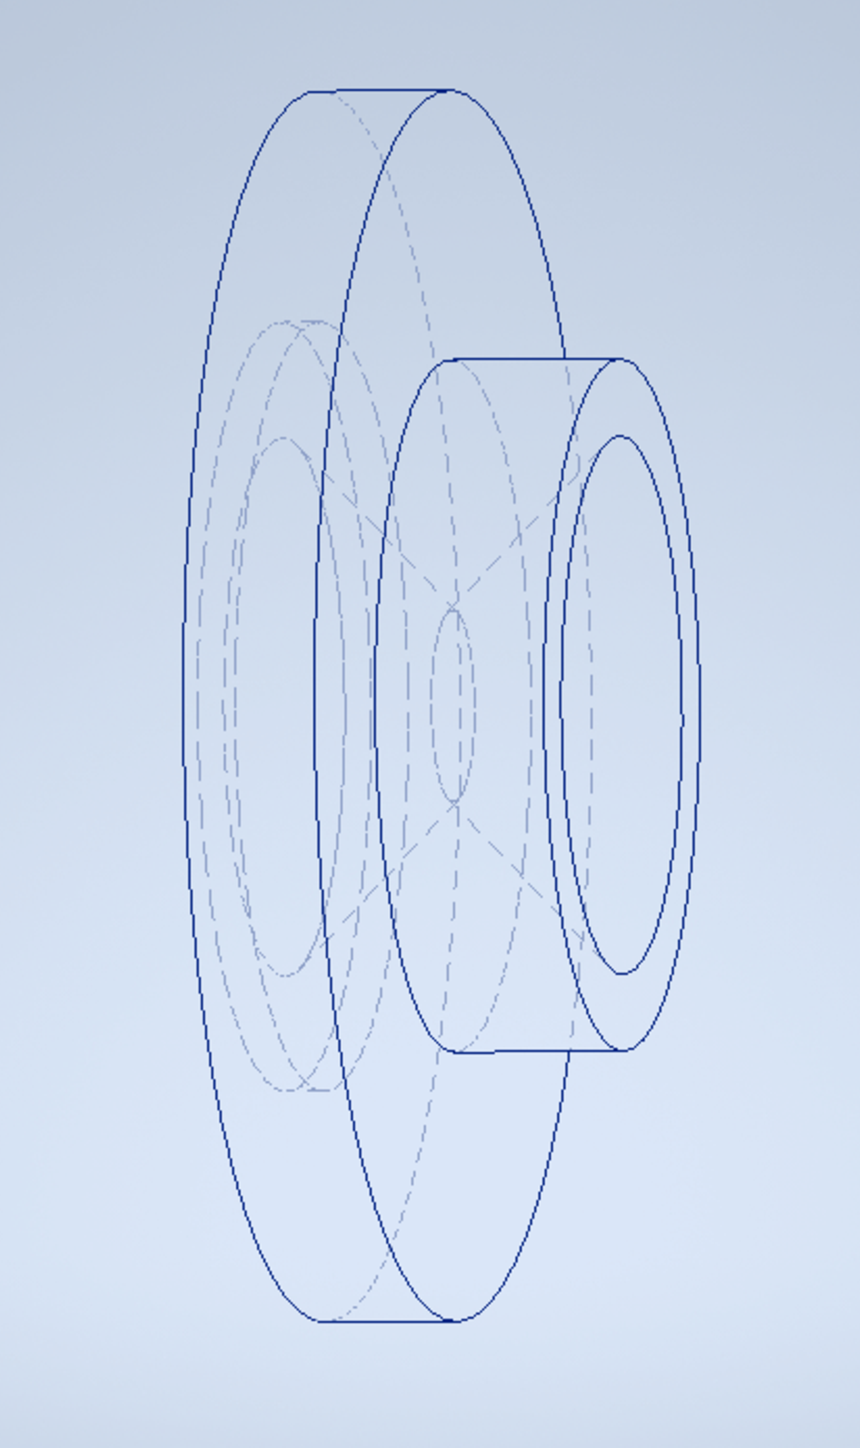
\includegraphics[scale=0.2]{assets/newchamfer.pdf}
    \end{center}

    \begin{center}  
        Old geometry \hspace*{2em} New Geometry
    \end{center}
        
\end{frame}

\end{document}